% -*- TeX:SI -*-
% slovene sub-mode for spell check
% ----------------------------------------------------------------------
%  Predloga za obliko in navodila za pisanje diplomskih nalog v LaTex-u

%  Univerza v Ljubljani, Fakulteta za elektrotehniko

%  zbral in uredil Roman Kamnik, junij 2013

% ----------------------------------------------------------------------

\documentclass[a4paper,twoside,openright,12pt]{book}
\usepackage[cp1250]{inputenc}  %Kodna stran za Windows okolje, za linux je kodna stran latin2
\usepackage[slovene]{babel}    % pravila za slovensko deljenje besed
\usepackage[pdftex]{UNI-LJ-FE-Diploma} %Stil za diplome na Fakulteti za elektrotehniko (za pdfTeX v MkiTex)
%\usepackage[pctex]{UNI-LJ-FE-Diploma} %Stil za diplome na Fakulteti za elektrotehniko  (za pcTex)
\usepackage{graphicx}

\usepackage{tikz}
\usetikzlibrary{calc}
\usepackage{subcaption} 

\newcommand{\magnet}[5]{% xsredisce, ysredisce, zasuk besedilo v srediscu najb bo crta ali ne
 \pgfmathsetmacro{\Cosa}{cos(#3)}
 \pgfmathsetmacro{\Sina}{sin(#3)}
\draw (#1,#2) circle (2);
\draw (#1+ -2.0 *#5* \Cosa  ,#2 -2.0 *#5* \Sina )--(#1+2.0 *#5* \Cosa , #2+2.0 *#5* \Sina );
\node at (#1-1.6*\Sina ,#2+1.6*\Cosa ){\rotatebox{#3}{N}};
\node at (#1+1.6*\Sina ,#2-1.6*\Cosa  ){\rotatebox{#3}{S}};
\fill (#1,#2) circle [radius=1pt] node [anchor=north east]{#4};
}


\newcommand{\senzorja}[4]{% xsredisce, ysredisce, zasuk
 \pgfmathsetmacro{\Cosb}{cos(#3)}
 \pgfmathsetmacro{\Sinb}{sin(#3)}



\hall{#1+2.4*\Cosb }{#2+2.4*\Sinb }{#3}
\hall{#1-2.4*\Sinb}{#2+2.4*\Cosb}{#3}
\fill (#1,#2) circle [radius=1pt] node [anchor=south east]{#4};

\draw [dashed, thick](#1,#2)--(#1+2.2*\Cosb ,#2+2.2*\Sinb );
\draw [dashed, thick](#1,#2)--(#1-2.2*\Sinb ,#2+2.2*\Cosb );
}

\newcommand{\hall}[3]{

 \pgfmathsetmacro{\Cosd}{cos(#3)}
 \pgfmathsetmacro{\Sind}{sin(#3)}
 
\draw 
(#1 - 0.2 * \Sind -0.2 * \Cosd  ,#2 + 0.2 * \Cosd -0.2 *\Sind )--
(#1 - 0.2 * \Sind +0.2 * \Cosd  ,#2 + 0.2 * \Cosd +0.2 *\Sind )--
(#1 + 0.2 * \Sind +0.2 * \Cosd  ,#2 - 0.2 * \Cosd +0.2 *\Sind )--
(#1 + 0.2 * \Sind -0.2 * \Cosd  ,#2 - 0.2 * \Cosd -0.2 *\Sind )--
(#1 - 0.2 * \Sind -0.2 * \Cosd  ,#2 + 0.2 * \Cosd -0.2 *\Sind );

\draw (#1-0.1*\Cosd -0.1*\Sind,#2+0.1*\Cosd-0.1*\Sind) --(#1+0.1*\Cosd +0.1*\Sind,#2-0.1*\Cosd+0.1*\Sind);
\draw (#1+0.1*\Cosd -0.1*\Sind,#2+0.1*\Cosd+0.1*\Sind)-- (#1-0.1*\Cosd +0.1*\Sind,#2-0.1*\Cosd-0.1*\Sind);
}
\newcommand{\CaCS}[3]{
	
	\draw [<->](-#1+#2,#3)--(#1+#2,0+#3) node[anchor=north]{$x$};
	\draw [<->](#2,-#1+#3)--(0+#2,#1+#3) node[anchor=east]{$y$};
	
	}

%*************************** PRILAGODITVE *****************************
% mapa s slikami
\potgrafike{./Slike/}
%prilagoditev levega roba sodih strani. �e se pri dvostranskem tisku robovi ne umemajo se lahko pove�a ali pomanj�a
\zamaknirobsodihstrani{0mm}

%*************************** NASLOVNA STRAN *****************************
\naslov{Vpliv stat�ne in dinami�ne ekscentri�nosti na napako senzorja RM44, u�inkovitost kalibracije in robustnost kalibracije na harmonske oscilacije mehanske hitrosti}
\avtor{Mitja Ali�} \univerza{Univerza v Ljubljani}
\fakulteta{Fakulteta za elektrotehniko}
\delo{Magistrsko delo}
%\delo{Diplomsko delo visoko�olskega strokovnega �tudija}
\date{Ljubljana, 2017}
\mentor{doc. dr. Mitja Nemec}
%\somentor{prof. dr. Ime Priimek}
\begin{document}

%------------------------ ZA�ETNI DEL -----------------------------------
%\frontmatter
%%------------------------------------------------------------------------
%
%
%%************************ NASLOVNA STRAN ********************************
%\maketitle
%
%
%%*************************** ZAHVALA ************************************
%\zahvala V zahvali se kandidati zahvali mentorju in poimensko tudi
%vsem sodelavcem in prijateljem, ki so pomagali in prispevali pri
%delu v laboratoriju, na ra�unalniku, v delavnici, pri tehni�ni
%izdelavi dela in drugje.
%
%
%%*************************** VSEBINA *************************************
%\tableofcontents
%
%%*************************** SEZNAM SLIK in TABEL  ***********************
%\seznamslik
%\seznamtabel
%
%%***************************  SEZNAM UPORABLJENIH SIMBOLOV  **************
%
%\seznamsimbolov
%
%V pri�ujo�em zaklju�nem delu so uporabljeni naslednje veli�ine in
%simboli:
%
%\begin{table}[h]
%\centering
%%\begin{footnotesize}
%\begin{tabular}{l l l l}
% \hline \multicolumn{2}{c}{\bf{Veli�ina / oznaka}} & \multicolumn{2}{c}{\bf{Enota}}  \\
% \hline
%Ime & Simbol & Ime & Simbol \\
% \hline
% �as & $t$  & sekunda & s \\
% frekvenca & $f$  & Hertz & Hz \\
% tlak & $p$  & Pascal & Pa \\
% sila vzgona & $\textbf{\textit{f}}_\text{vz}$  & Newton & N \\
% gostota & $\rho$  & - & kg/m$^3$ \\
% masa telesa  & $m_\text{t}$  & kilogram & kg \\
% vhodna napestost & $U_\text{vh}$ & volt  & V \\
% Jacobijeva matrika & $\mathbf{J}$  & - & - \\
%  \hline
%\end{tabular}
%%\end{footnotesize}
%  \caption{Veli�ine in simboli}
%  \label{prebojne_trdnosti}
%\end{table}
%
%
%
%%------------------------ GLAVNI DEL ------------------------------------
%\mainmatter
%%-------------------------------------------------------------------------
%
%
%%********************* POVZETEK V SLOVEN��INI ****************************
%\povzetek
%
%V pri�ujo�em delu so predstavljena navodila za izdelavo 
%
%\kljucnebesede beseda1, beseda2, beseda3
%
%
%%*************************** POVZETEK V ANGLE��INI ***********************
%\abstract
%
%The thesis addresses ...
%
%\keywords word1, word2, word3
%
%
%%***************************** UVOD **************************************
%\chapter{Uvod} \label{uvod}
%
%Uvod v zaklju�no delo ima namen, da uvede bralca v tematiko
%zaklju�nega dela. V njem kandidat raz�leni zahteve in cilje
%zaklju�nega dela, po literaturi povzame znane 
%re"sitve in oceni
%njihov pomen za zaklju�no delo. Sklicevanje na literaturo se v
%besedilu ozna�i s "stevilko v oglatem oklepaju, ki jo ima ta v
%seznamu uporabljenih virov, in po potrebi navede strani, npr.
%\cite{miklavvcivc2010objavljanje} ali \cite[stran 520 -
%534]{juvznivc1992diplomska}.
%
%%*********************** OSREDNJA POGLAVJA ********************************
%\chapter{Izbira teme zaklju�nega dela} \label{izbira_teme}
%
%\chapter{Princip delovanja senzorja RM44}
%
%
%
%
%\chapter{Dolo"canje napake s simulacijo}


\chapter{Uvod}

V dana"snjem "casu elektromotorski pogoni vse hitreje nadome"scajo druge oblike ustvarjanja mehanskega dela. Zahteve po "cim hitrej"si regulaciji in zaneslivosti pogona so "cedalje vi"sje. V pogonih se "zeli dose"ci tudi "cim vi"sji izkoristek. Za doseganje uspe"snega obratovanja elektromotorskega pogona se potrebuje dober in zanesljiv dajalnik pozicije. 
Dejalnike delimo na linearne dajalnike in dajalnike zasuka oz. rotacije. Tu se bom osredoto"cil na rotacijske dajalnike pozicije. Ti so lahko montirani na poljubnem mestu na osi (angl.: through hole), ali le na koncu osi (ang.: On-axis).

%analogni-digitalni senzorji
%relativni absolutni dajalniki

Vsak dajalnik ima to"cnost, katero dose"ze, "ce je pravilno montiran. naapka nepravilne montaze je odvisna od nepravilno postavljenega aktuatorja na osi pogona, ali nepravilno montiranega senzorja. V tem delu bom analiziral kako se napaka ....

V tem delu se bom osredoto"cil na dajalnik RM44, ki ga bom namerno 



Dajalnike lo"cimo tudi glede na uporabljen princip zaznavanja premika. Poznamo magnetne, opti"cne, induktivne in druge. 
Dejalniki se razlikujejo tudi na izodne signale.




\chapter{Dajalniki pozicije RM44}

Dajalnik pozicije RM44 je produkt podjetja RLS merilna tehnika d.o.o. kratica RLS pomeni rotacijski in linearni senzorji zasuka (ang.: Rotary and Linear motion Sensors). Podjetje proizvaja merilnike na podlagi merjenja magnetnega polja. Dajalnik pozicije RM44 spada v dru"zio enkoderjev montiranih na koncu osi rotirajo"ce gredi (ang.: On-axis). Na rotirajo"co os je pritrjen cilindri"cni magnet, ki je diametralno magnetiziran. %(dodaj sliko iz diplome barbare na strani 22 )
Senzor je sestavljen iz "cipa AM8192B, v katerem so vgrajene Hallove sonde za merjenje pravokotne komponente magnetnega polja, magneta montiranega na os pogona. Izhod senzorja je lahko analogen v obliki dveh signalov sinusa in kosinusa. Izhod senzorja je lahko inkrementalni, ki poda relativno spremembo pozicije ter smer premikanja. Senzor lahko prika"ze tudi absolutno vrednost pozicije. Njegova resolucija je nastavljiva med 320 in 8192 pozicij na obrat.

\chapter{Analiti"cna izpeljava dinami"cne in stati"cne eks"centri"cnosti}

Napake so prisotne pravzaprav pri vsakem senzorju. V tem poglavju bom analiti"cno prikazal vpliv napak omenjenih ekscentri"cnosti, ki se pojavijo ob nepravilni monta"zi senzorja. Njuna vpliva ra"zli"cno vplivata na napako zato ju bom obravnaval posami"cno. V delu sem predpostavil, da se izmiki iz idealne pozicije izmikajo le v smeri x in y. Napaka se pojavi tudi ob premiku v smeri z vendar tega tu nebom obravnaval.
 Zaradi narave problema je smiselno uporabiti kartezi"ni koordinatni sistem. V izpeljavah bom predpostavil, da so izmiki majhni. Najprej bom izpeljal po ka"sni trajetoriji se giblje posamezna Hallova sonda. Iz znane tretnutne lokacije Hallove sonde bom lahko izra"cunal vrednost B komponente ki jo meri posamezna Hallova sonda. Pri analiti"cni izpeljavi bom predopstavil, da je polje ob majhnih odmikih linearno in ustreza enacbi polja $B(x,y)=k \cdot x$.  Nato bom analiti"cno izrazil vrednost kota, ki predstavlja izhod senzorja.



\section{Za"cetna pozicija senzorjev}

Za dolo"canje kota med vektorjem ki ka"ze v smeri x-os (\textbf{$1_x$}) in vektorjem med koordinatnim izhodiscem in poljubno to"cko v koordinatnem sistemu, je potrebno poznati poznati le polo"zaj to"cke. Primer je podan na sliki \ref{fig:dolocitev_kota}. Kot $\varphi$ dolo"cimo preko trigonometri"cne funkcije $\arctan$: $$\varphi=\arctan\frac{y_0}{x_0}$$



\begin{figure}[h!]
	\centering
	\begin{tikzpicture}[scale=4]
	\CaCS{0.75}{0}{0}
	\draw [->,thick](0,0)--(-0.5,0.2855);
	\draw (0.15,0) arc (0:150:0.15);
	\node at (0.05,0.05){$\varphi$};
%	\node at (-0.5,0.285) {\textbullet};
	\node at (-0.32,0.35) {($x_0$,$y_0$)};
	\end{tikzpicture}
	\caption{Slika za pomo"c pri dolo"canju kota}
	\label{fig:dolocitev_kota}
\end{figure}


Za dolo"citev kota $\varphi$  je dovolj poznati "ze projekciji vektorja na koordinatni osi(slika \ref{fig:dolocitev_kota_2}),

\begin{figure}[h!]
	\centering
	\begin{tikzpicture}[scale=4]
	\CaCS{0.75}{0}{0}
	\draw [->,thick](0,0)--(-0.5,0.2855);
	\draw (0.15,0) arc (0:150:0.15);
	\node at (0.05,0.05){$\varphi$};
	\draw [dashed] (-0.5,0.2855)--(-0.5,0);
	\draw [dashed] (-0.5,0.2855)--(0,0.2855);
	%	\node at (-0.5,0.285) {\textbullet};
%	\node at (-0.32,0.35) {($x_0$,$y_0$)};
	\node at(-0.5,-0.1){$x_0$} ;
	\node at(0.1,0.2855){$y_0$};
	\end{tikzpicture}
	\caption{Slika za pomo"c pri dolo"canju kota}
	\label{fig:dolocitev_kota_2}
\end{figure}


"Ce poznamo le projekciji to"cke na koordinatni osi, je to zadosten pogoj za dolo"citev kota $\varphi$.
Za dolo"citev kota zasuka v idealnih pogojih, kot je predpostavka, da je polje linearno, sta dovolj dve Hallovi sondi, ki sta prostorsko zamaknjeni za 90$^\circ$ (Slika \ref{fig:zacetna_postavitev_sond}).

Za"cetni lokaciji sond enostavmo postavimo na koordinatni osi in s tem ustre"zemo pogoju po prostorskem zasuku med sondama. Sondi postavimo na razdaljo $r_0$ od koordinatnega izhodi"s"ca. S tem dobimo za"cetni lokaciji Hallovih sond $\mathrm{H}_1(x_0, y_0)=(r_0, 0)$, $\mathrm{H}_2(x_0, y_0)=(0, r_0)$.



\begin{figure}[h!]
	\centering
	\begin{tikzpicture}[scale=1]
	\CaCS{3}{0}{0}
	\senzorja{0}{0}{0}{}
%	\magnet {0} {0} {10}{ }{0}
	\node at (2.0,-0.5){$\mathrm{H}_1(r_0,0)$};
	\node at (-1,2.3){$\mathrm{H}_2(0, r_0)$};
	\end{tikzpicture}
	\caption{Za"cetna postavitev Hallovih sond}
	\label{fig:zacetna_postavitev_sond}
\end{figure}


\section{Zasuk magneta}

Z zasukom magneta za kot $\theta$ se na mestu, kjer merimo magnetno polje, polje spremni. Polje bi se spremnilo enako "ce bi nad magnetom  zasukali senzor za kot $-\theta$. Hallova sonda z za"cetno lokacijo ($x_0, y_0$) bi se po kro"znici premaknila v novo lokacijo($\mathrm{x, y}$):
\begin{equation}
\label{eq:osnovni_zasuk}
\begin{bmatrix}
x\\y
\end{bmatrix}= \begin{bmatrix}
\cos (-\theta)& -\sin(-\theta)\\ \sin( -\theta)& \cos (-\theta)
\end{bmatrix}
\cdot
\begin{bmatrix}
x_0\\y_0
\end{bmatrix}
\end{equation}
Z upo"stevanjem da je funkcija sinus liha in funkcija kosinus soda, se izra"cun v ena"cbi \ref{eq:osnovni_zasuk} poenostavi v:
\begin{equation}
\label{eq:osnovni_zasuk_popravljena_rot}
\begin{bmatrix}
x\\y
\end{bmatrix}= \begin{bmatrix}
\cos (\theta)& \sin(\theta)\\ -\sin( \theta)& \cos (\theta)
\end{bmatrix}
\cdot
\begin{bmatrix}
x_0\\y_0
\end{bmatrix}
\end{equation}




\begin{figure}[h!]
	\begin{subfigure}[b]{0.5\textwidth}
		\centering
		\resizebox{\linewidth}{!}{
			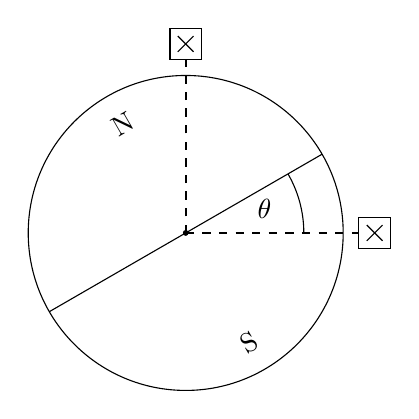
\begin{tikzpicture}
	\senzorja{0}{0}{0}{}
	\magnet {0} {0} {30}{ }{1}
	\draw (1.5,0) arc (0:30:1.5);
	\node at (1,0.3){$\theta$};
			\end{tikzpicture}
		}
		\caption{Zasukan magnet za kot $\mathrm{\theta}$}
		\label{fig:subfig8}
	\end{subfigure}
	\begin{subfigure}[b]{0.5\textwidth}
		\centering
		\resizebox{\linewidth}{!}{
			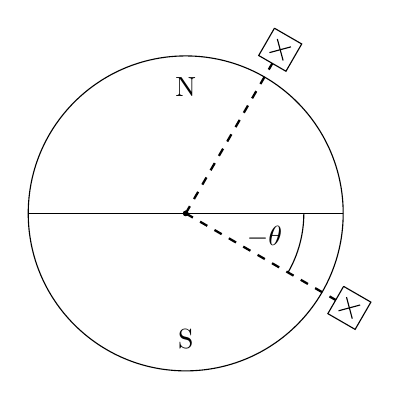
\begin{tikzpicture}

				\senzorja{8}{0}{-30}{}
				\magnet {8} {0} {0}{ }{1}
				\draw (1.5+8,0) arc (0:-30:1.5);
				\node at (1+8,-0.3){$-\theta$};
			\end{tikzpicture}
		}
		\caption{Zasukan senzor za kot $\mathrm{-\theta}$}   
		\label{fig:subfig9}
	\end{subfigure}

	\caption{Hallovi sondi se glede na magnet nahajati na enaki lokaciji}
	\label{fig:subfig1.a.4}
\end{figure}

Ko zavrtimo senzor okoli magneta pri tem pomeri polje. Ker sem predpostavil linearno polje, ga predstavim s izrazom 
\begin{equation}
\label{eq:enacba_polja}
B(x,y)=k \cdot x
\end{equation}
Za poenostavitev vzemimo $k=1$. S tem se ena"cba \ref{eq:enacba_polja} poenostavi v:
\begin{equation}
\label{eq:enacba_polja_2}
B(x,y)=x
\end{equation}


Polje ki ga pomeri posamezna sonda dobimo z upostevanjem ena"cb \ref{eq:osnovni_zasuk_popravljena_rot} in \ref{eq:enacba_polja_2}.
\begin{equation}
B_{H_1}(\theta)=r_0\cdot \cos \theta
\end{equation}
\begin{equation}
B_{H_2}(\theta)=r_0\cdot \sin \theta
\end{equation}

%\slikaeps{magnetno polje ki ga pomeriti sondi ko je vse scentrirano}{B1B2_brez_eks}




%Zaradi majhnih odmikov lahko predpostavim, da je pravokotna komponenta vektorja gostote magnetnega pretoka(vektor \textbf{B}) linearna. S tem se izpeljava za dolo"canje pozicije, poenostavi. Kasneje bom predstavil tudi na"cin kako pridobiti vredn ost \textbf{B} realnega polja. Predpostavil bom tudi da je senzor za mejenje pozicije sestavljen le iz dveh Hallovih sond, pri kateri je druga sonda fazno premaknjena za 90$^\circ$. 
%slika kjer je narisano linearno polje





%\begin{figure}
%\centering
%\begin{tikzpicture}[scale=1]
%\magnet {0} {0} {10}{ }{1}
%\senzorja{0}{0.5}{0}{$S_h$}
%\draw (0,0) circle (0.5);
%\senzorja{-0.35}{0.35}{45}{$S_h$}


%\end{tikzpicture}
%\caption{Prikaz navora v odvistnosti od komponent toka }
%
%\label{fig:navor}
%\end{figure}
%izpeljava ekscentricnosti za 1 senzor [x0,y0]

%\section{izpeljava stati"cne ekscentri"cnosti}
%Napises da je senzor izmaknjen iz centra magneta in sredisce senzorja opise kroznico
%
%
%
%
%\section{izpeljava dinami"cne ekscentri"cnosti}
%napisi da je magnet izmaknjen senzor pa zavrtis okoli sredisca senzorja






%\section{Rezultati simulacij}
%
%\chapter{Zaklju�ek} \label{zakljucek}
%
%
%


\end{document}
